\documentclass[12pt, letterpaper]{article}

% --- PAQUETES DE IDIOMA Y FORMATO ---
\usepackage[utf8]{inputenc}
\usepackage[spanish]{babel}
\usepackage[margin=2.5cm]{geometry}
\usepackage{graphicx} 
\usepackage{hyperref} 
\usepackage{xcolor}   
\usepackage{listings}
\usepackage{booktabs} 
\usepackage{float}
\usepackage{tcolorbox} % Para las cajas de advertencia

% --- COLORES PERSONALIZADOS ---
\definecolor{primary}{RGB}{0, 51, 102}
\definecolor{warningred}{RGB}{204, 0, 0}
\definecolor{lightgray}{RGB}{240, 240, 240}

% --- CONFIGURACIÓN PARA EL CÓDIGO JAVA Y TEXTO PLANO ---
\definecolor{codegreen}{rgb}{0,0.6,0}
\definecolor{codegray}{rgb}{0.5,0.5,0.5}
\definecolor{codepurple}{rgb}{0.58,0,0.82}
\definecolor{backcolour}{rgb}{0.95,0.95,0.92}

\lstdefinestyle{mystyle}{
	backgroundcolor=\color{backcolour},   
	commentstyle=\color{codegreen},
	keywordstyle=\color{magenta},
	numberstyle=\tiny\color{codegray},
	stringstyle=\color{codepurple},
	basicstyle=\ttfamily\footnotesize,
	breakatwhitespace=false,         
	breaklines=true,                 
	captionpos=b,                    
	keepspaces=true,                 
	numbers=left,             
	numbersep=5pt,                  
	showspaces=false,                
	showstringspaces=false,
	showtabs=false,                  
	tabsize=2
}
\lstset{style=mystyle}

% --- INICIO DEL DOCUMENTO ---
\begin{document}
	
	% --- PORTADA ---
	\begin{titlepage}
		\centering
		\vspace*{0.5cm}
		
		
\includegraphics[width=2.8cm]{logo_unam.png} 
		\hfill
		
\includegraphics[width=2.8cm]{logo_fi.png} 
		\\[1cm] 
		
		{\Huge \textbf{Universidad Nacional Autónoma de México}}\\[0.5cm]
		{\LARGE \textbf{Facultad de Ingeniería}}\\[1cm]
		
		{\Large Asignatura: Programación Orientada a Objetos}\\[0.5cm]
		{\Large Proyecto: Sistema de Gestión y Reservación de Vuelos}\\[1cm]
		
		% Título del Reporte
		\rule{\linewidth}{0.5mm} \\[0.4cm]
		{ \huge \bfseries Aeroviajes: \\ Manual de Usuario y Guía Operativa (v 1.0) }\\[0.4cm]
		\rule{\linewidth}{0.5mm} \\[1.5cm] 
		
		\begin{flushleft}
			\Large \textbf{Equipo de Desarrollo:}\\
			\vspace{0.3cm}
			\normalsize
			$\bullet$ Francisco José Coutiño Morales\\ 
			$\bullet$ Ernesto Flamenco Villaseñor\\
		\end{flushleft}
		
		\vfill 
		
		{\large 27 de mayo de 2026} 
	\end{titlepage}
	
	% --- ÍNDICE ---
	\newpage
	\tableofcontents
	\newpage
	
	% =========================================================================
	% --- SECCIÓN 1: INTRODUCCIÓN ---
	% =========================================================================
	\section{Introducción}
	Bienvenido al Manual de Usuario del sistema \textbf{Aeroviajes}. Este software ha sido diseñado bajo una arquitectura de Interfaz Gráfica de Usuario (GUI) en Java Swing para gestionar la reservación de vuelos comerciales en tiempo real, de manera intuitiva y segura.
	
	Este manual está dirigido al usuario final del sistema —ya sea un \textbf{cliente} que desea adquirir un boleto, o un \textbf{administrador} que opera el catálogo de vuelos— así como al profesor de la asignatura \textbf{Ing. Edgar Tista}, proporcionando las instrucciones paso a paso para la correcta interacción con el sistema y las advertencias de seguridad necesarias para evitar interrupciones causadas por entradas inválidas.
	
	A diferencia de aplicaciones de consola, Aeroviajes se navega íntegramente con el mouse mediante botones, formularios y tablas. Toda la información se persiste automáticamente en disco, por lo que los usuarios registrados, vuelos disponibles y reservas confirmadas sobreviven al cierre y reinicio del programa.
	
	% =========================================================================
	% --- SECCIÓN 2: CONCEPTOS CLAVE DEL SISTEMA ---
	% =========================================================================
	\section{Conceptos Clave del Sistema}
	Para operar el sistema correctamente, el usuario debe comprender cómo el software clasifica la información. Aeroviajes maneja \textbf{dos roles} claramente diferenciados, cada uno con un menú y permisos propios:
	
	\begin{itemize}
		\item \textbf{Cliente:} Persona que se registra en el sistema para consultar el catálogo de vuelos y realizar compras de boletos. Cada cliente posee un \textbf{correo electrónico único} que actúa como su identificador, y una \textbf{contraseña generada automáticamente por el sistema} al momento del registro.
		\item \textbf{Administrador:} Operador del sistema con permisos elevados. Puede agregar y eliminar vuelos del catálogo, así como ver y eliminar usuarios registrados. El sistema crea automáticamente un administrador por defecto en la primera ejecución, con credenciales preestablecidas.
	\end{itemize}
	
	El sistema también maneja los siguientes objetos del negocio:
	
	\begin{itemize}
		\item \textbf{Vuelo:} Trayecto aéreo identificado por un ID único (ej. \texttt{AM404}), una aerolínea, un aeropuerto de origen y otro de destino (representados por su código IATA de tres letras), una fecha de salida, un precio y una capacidad de asientos.
		\item \textbf{Reserva:} Contrato generado al momento de la compra. Cada reserva tiene un identificador único (ej. \texttt{R-462AAC}), un asiento asignado y un estado (\texttt{CONFIRMADA}).
		\item \textbf{Boleto (Ticket):} Documento generado automáticamente al confirmar una reserva. El sistema lo crea en un hilo separado (en segundo plano), por lo que el usuario no tiene que esperar a que finalice el proceso para seguir navegando. El boleto puede consultarse y descargarse como archivo de texto.
	\end{itemize}
	
	% =========================================================================
	% --- SECCIÓN 3: INICIO DEL PROGRAMA ---
	% =========================================================================
	\section{Inicio del Programa}
	Al ejecutar la aplicación desde el IDE NetBeans (con la opción \texttt{Run Project} o la tecla \texttt{F6}), se desplegará la \textbf{Pantalla de Bienvenida} con tres opciones principales:
	
	\begin{figure}[H]
		\centering
		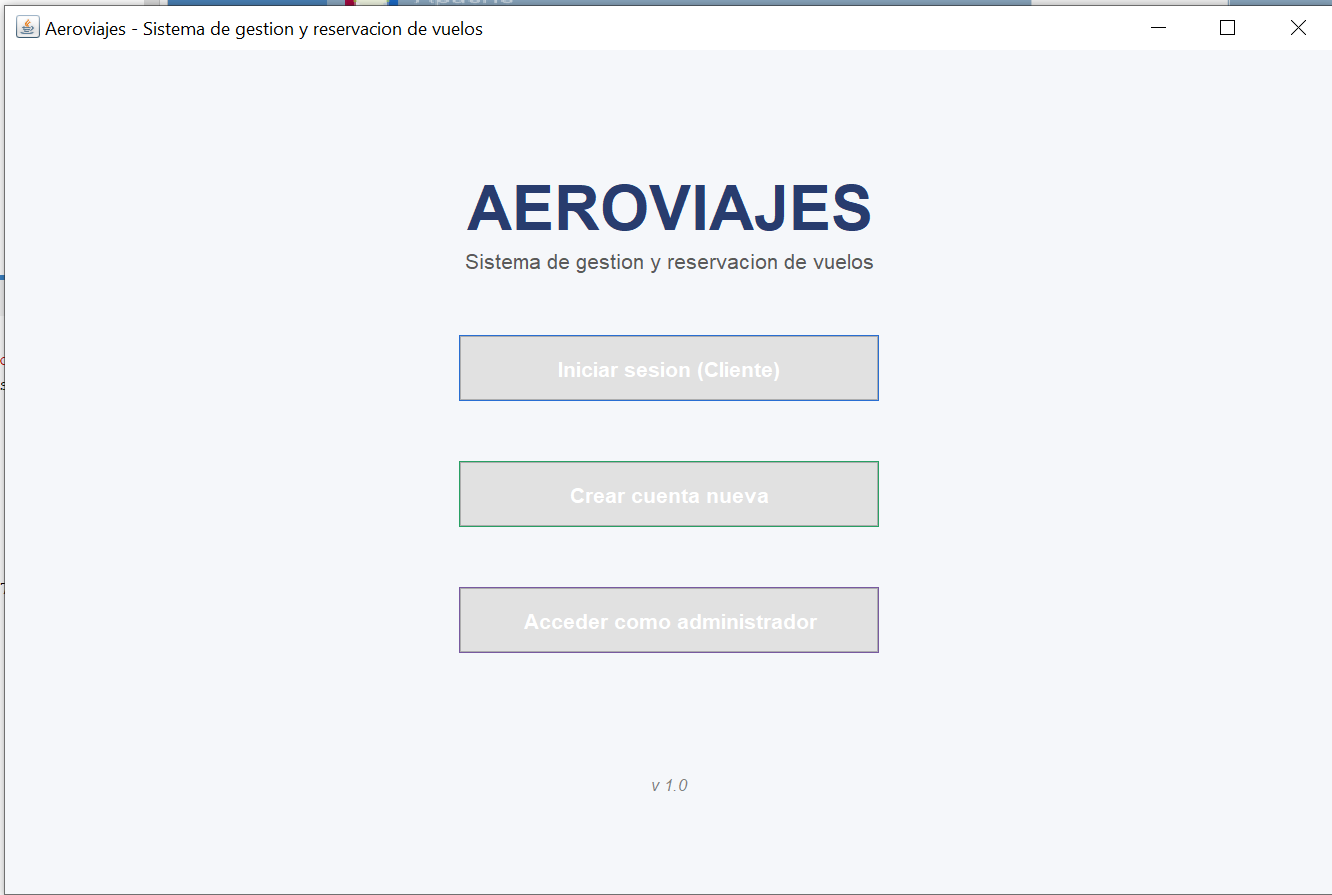
\includegraphics[width=0.85\textwidth]{Aeroviajes 1.png} 
		\caption{Pantalla de bienvenida del sistema Aeroviajes.}
		\label{fig:aeroviajes_1}
	\end{figure}
	
	Las tres opciones son:
	\begin{enumerate}
		\item \textbf{Iniciar sesión (Cliente):} Para usuarios ya registrados que desean acceder a su cuenta de cliente.
		\item \textbf{Crear cuenta nueva:} Para usuarios que ingresan al sistema por primera vez y desean registrarse como clientes.
		\item \textbf{Acceder como administrador:} Para el operador del sistema con permisos elevados.
	\end{enumerate}
	
	El usuario debe seleccionar la opción que corresponda con un clic.
	
	% =========================================================================
	% --- SECCIÓN 4: GUÍA DE OPERACIÓN CLIENTE ---
	% =========================================================================
	\section{Guía de Operación: Cliente}
	Esta sección describe el flujo completo de un cliente: desde su registro inicial hasta la descarga de su boleto de vuelo.
	
	\subsection{Registro de una Cuenta Nueva}
	Al pulsar el botón \textbf{``Crear cuenta nueva''} en la pantalla de bienvenida, se desplegará el formulario de registro. El usuario debe llenar los tres campos requeridos:
	
	\begin{figure}[H]
		\centering
		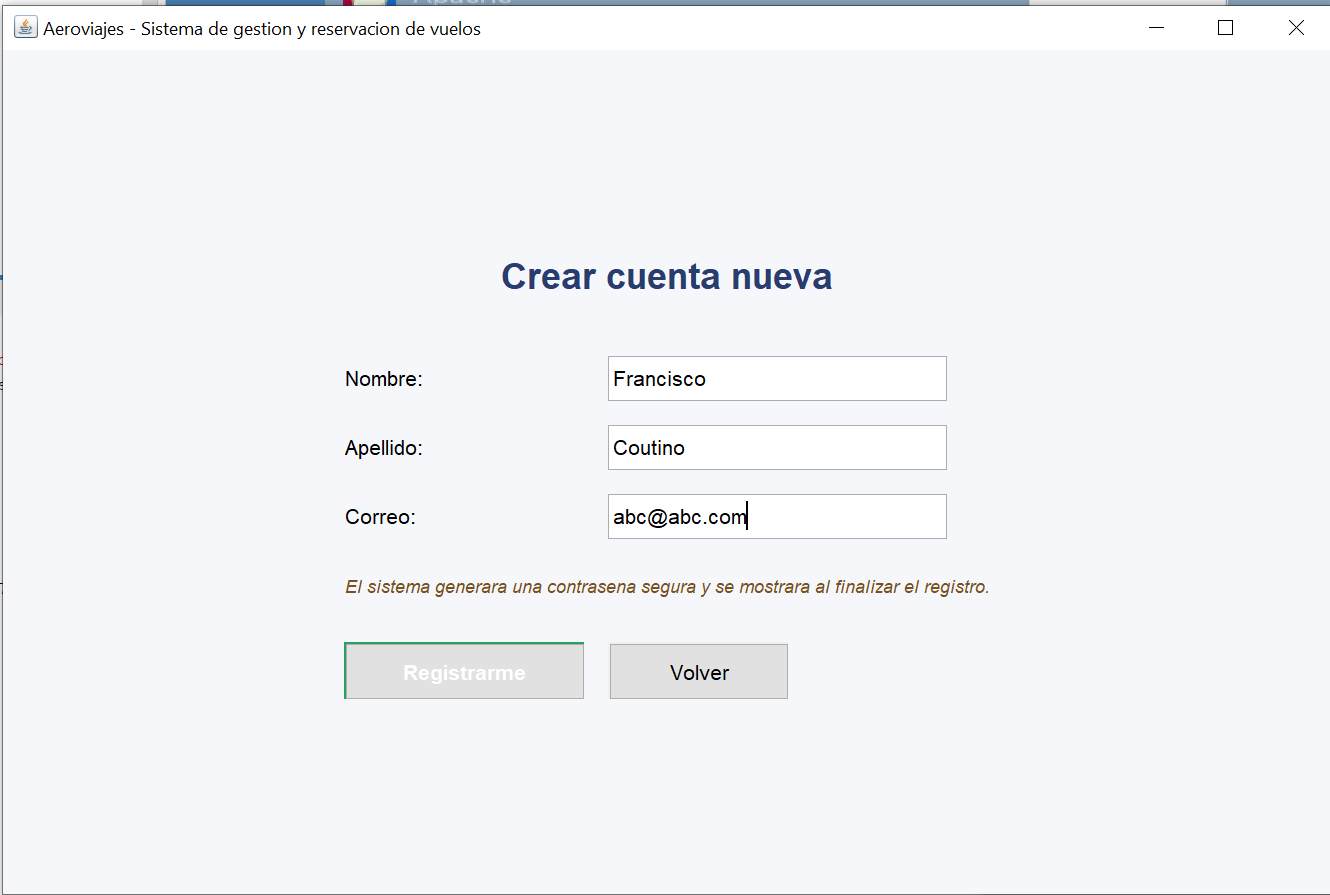
\includegraphics[width=0.7\textwidth]{Aeroviajes 2.png} 
		\caption{Formulario de registro de cliente.}
		\label{fig:aeroviajes_2}
	\end{figure}
	
	Los campos solicitados son:
	\begin{itemize}
		\item \textbf{Nombre:} Solo letras y espacios. Mínimo 2 caracteres.
		\item \textbf{Apellido:} Solo letras y espacios. Mínimo 2 caracteres.
		\item \textbf{Correo:} Debe seguir el formato estándar \texttt{usuario@dominio.com}. Será la \textbf{clave de acceso única} del cliente.
	\end{itemize}
	
	Una vez completados los datos, el usuario debe pulsar el botón \textbf{``Registrarme''}. El sistema validará automáticamente los formatos y, si todo es correcto, generará una contraseña segura aleatoria y la mostrará en un diálogo de confirmación:
	
	\begin{figure}[H]
		\centering
		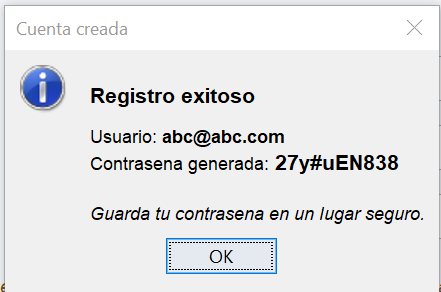
\includegraphics[width=0.6\textwidth]{Aeroviajes 3.png} 
		\caption{Diálogo de cuenta creada con contraseña generada automáticamente.}
		\label{fig:aeroviajes_3}
	\end{figure}
	
	\begin{quote}
		\textbf{IMPORTANTE:} El usuario debe anotar o memorizar la contraseña en el momento de su generación. El sistema no permite recuperarla posteriormente. Una vez cerrado el diálogo, la contraseña queda almacenada de forma encriptada y solo puede validarse, no leerse.
	\end{quote}
	
	La contraseña generada cumple con los siguientes criterios de seguridad:
	\begin{itemize}
		\item Exactamente 10 caracteres.
		\item Al menos una letra mayúscula, una minúscula, un dígito y un símbolo especial.
		\item Caracteres confusos (como \texttt{O}, \texttt{0}, \texttt{l}, \texttt{1}, \texttt{I}) excluidos para evitar errores de transcripción.
	\end{itemize}
	
	Tras cerrar el diálogo, el sistema regresa automáticamente a la pantalla de bienvenida.
	
	\subsection{Iniciar Sesión como Cliente}
	Para acceder al sistema con la cuenta recién creada, el usuario debe pulsar el botón \textbf{``Iniciar sesión (Cliente)''} en la pantalla de bienvenida. Se desplegará el formulario de autenticación:
	
	\begin{figure}[H]
		\centering
		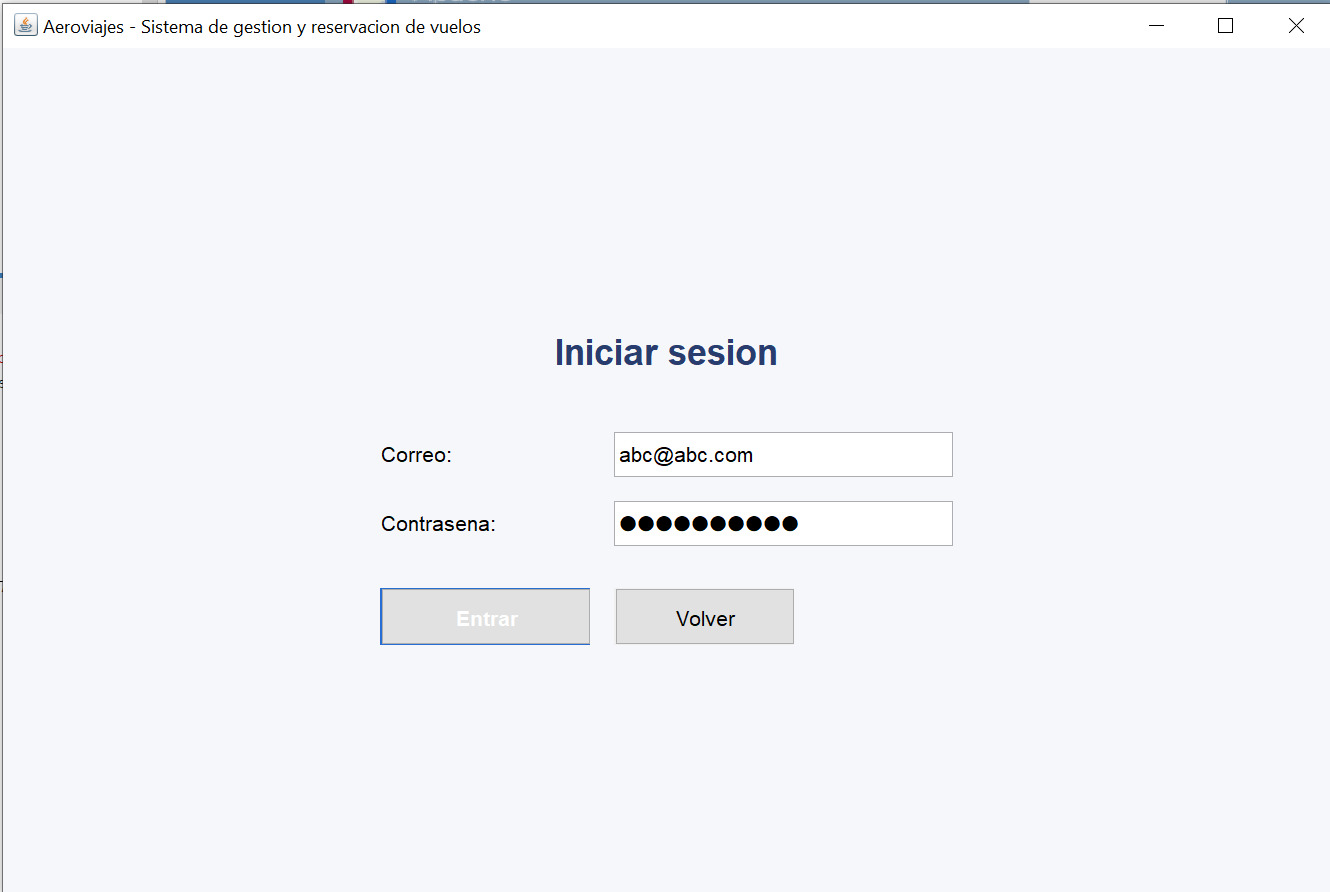
\includegraphics[width=0.7\textwidth]{Aeroviajes 4.png} 
		\caption{Pantalla de inicio de sesión.}
		\label{fig:aeroviajes_4}
	\end{figure}
	
	El usuario debe ingresar el correo y la contraseña generada al momento del registro, y pulsar \textbf{``Entrar''}. Si las credenciales son correctas, el sistema lo redirigirá al \textbf{Menú del Cliente}:
	
	\begin{figure}[H]
		\centering
		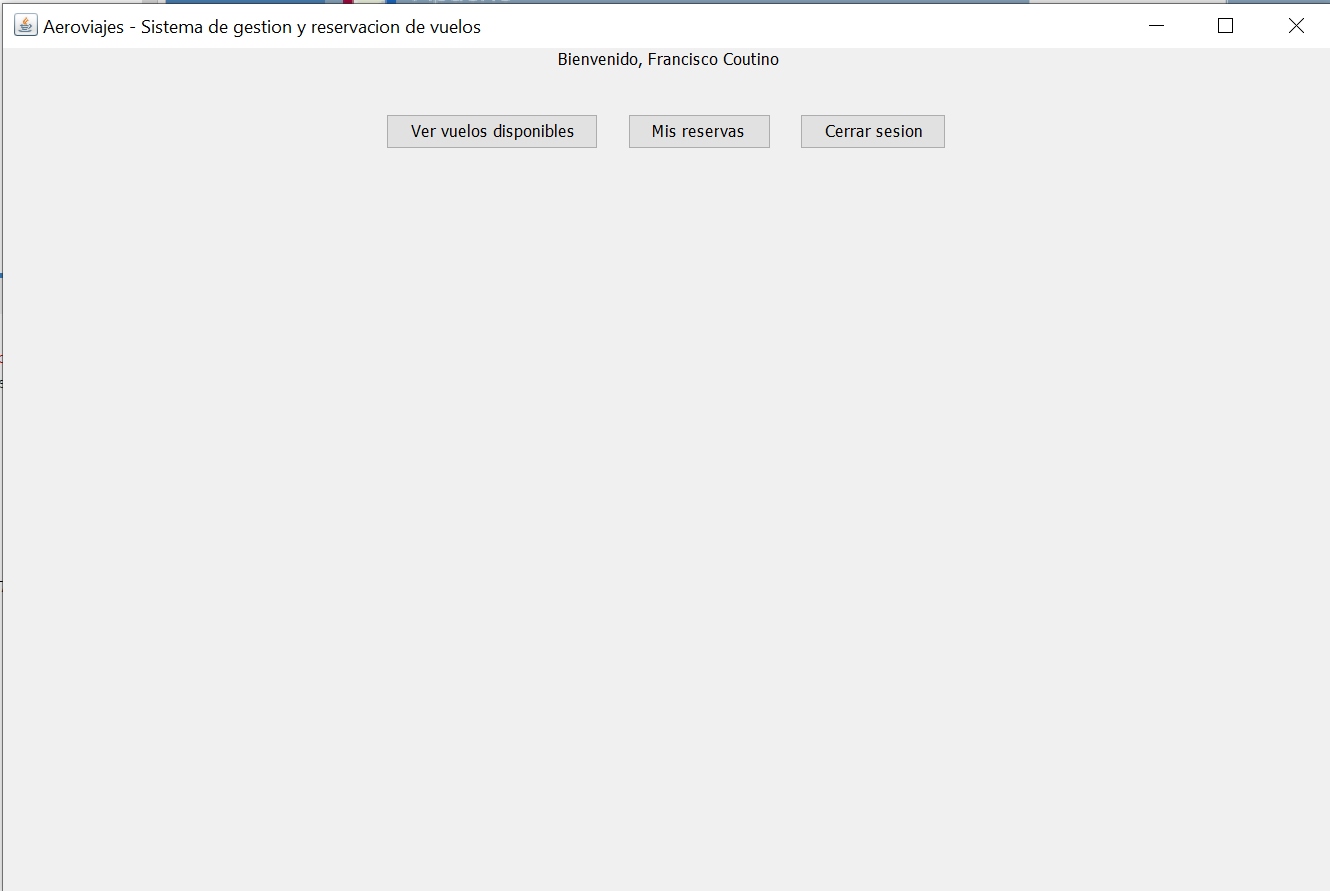
\includegraphics[width=0.8\textwidth]{Aeroviajes 5.png} 
		\caption{Menú principal del cliente tras iniciar sesión.}
		\label{fig:aeroviajes_5}
	\end{figure}
	
	El menú del cliente ofrece tres opciones principales:
	\begin{itemize}
		\item \textbf{Ver vuelos disponibles:} Lista todos los vuelos con asientos libres.
		\item \textbf{Mis reservas:} Consulta las reservas que el cliente ha realizado previamente.
		\item \textbf{Cerrar sesión:} Cierra la sesión activa y regresa a la pantalla de bienvenida.
	\end{itemize}
	
	\subsection{Consulta y Compra de Vuelos}
	Al pulsar \textbf{``Ver vuelos disponibles''}, el sistema despliega una tabla con todos los vuelos del catálogo que aún tienen asientos libres:
	
	\begin{figure}[H]
		\centering
		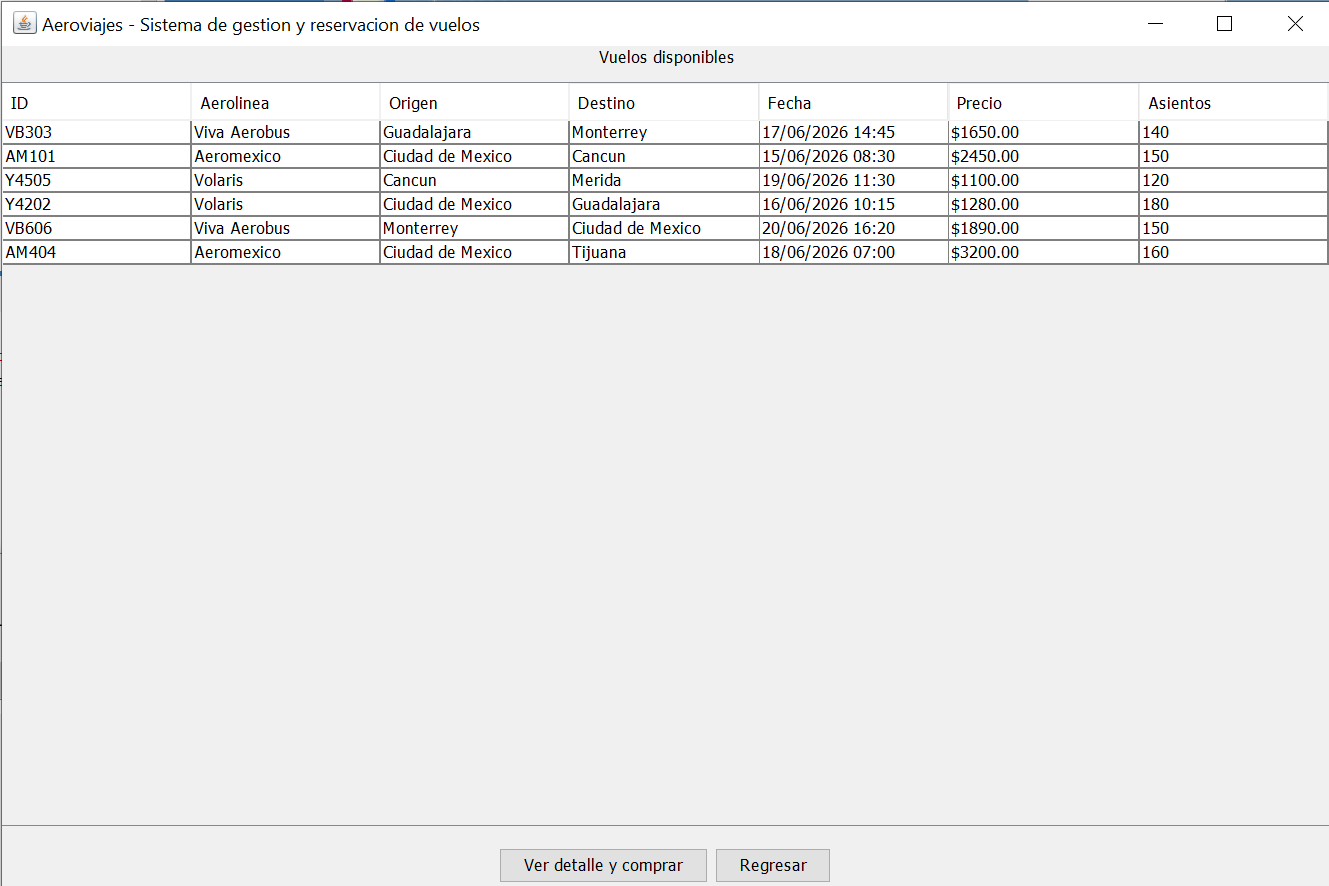
\includegraphics[width=0.85\textwidth]{Aeroviajes 6.png} 
		\caption{Tabla de vuelos disponibles.}
		\label{fig:aeroviajes_6}
	\end{figure}
	
	Cada fila de la tabla muestra:
	\begin{itemize}
		\item \textbf{ID:} Identificador único del vuelo (ej. \texttt{AM101}).
		\item \textbf{Aerolínea:} Compañía operadora del vuelo.
		\item \textbf{Origen y Destino:} Ciudades de salida y llegada.
		\item \textbf{Fecha:} Fecha y hora de salida en formato \texttt{dd/MM/yyyy HH:mm}.
		\item \textbf{Precio:} Costo del boleto en pesos mexicanos.
		\item \textbf{Asientos:} Capacidad disponible.
	\end{itemize}
	
	Para comprar un vuelo, el usuario debe:
	\begin{enumerate}
		\item Hacer \textbf{un clic} sobre la fila del vuelo deseado para seleccionarlo (se resaltará en azul).
		\item Pulsar el botón \textbf{``Ver detalle y comprar''} en la parte inferior.
	\end{enumerate}
	
	\begin{quote}
		Si el usuario pulsa ``Ver detalle y comprar'' sin haber seleccionado ningún vuelo, el sistema mostrará un mensaje de advertencia solicitando que primero seleccione un vuelo.
	\end{quote}
	
	El sistema mostrará entonces la pantalla de \textbf{Detalle del Vuelo}:
	
	\begin{figure}[H]
		\centering
		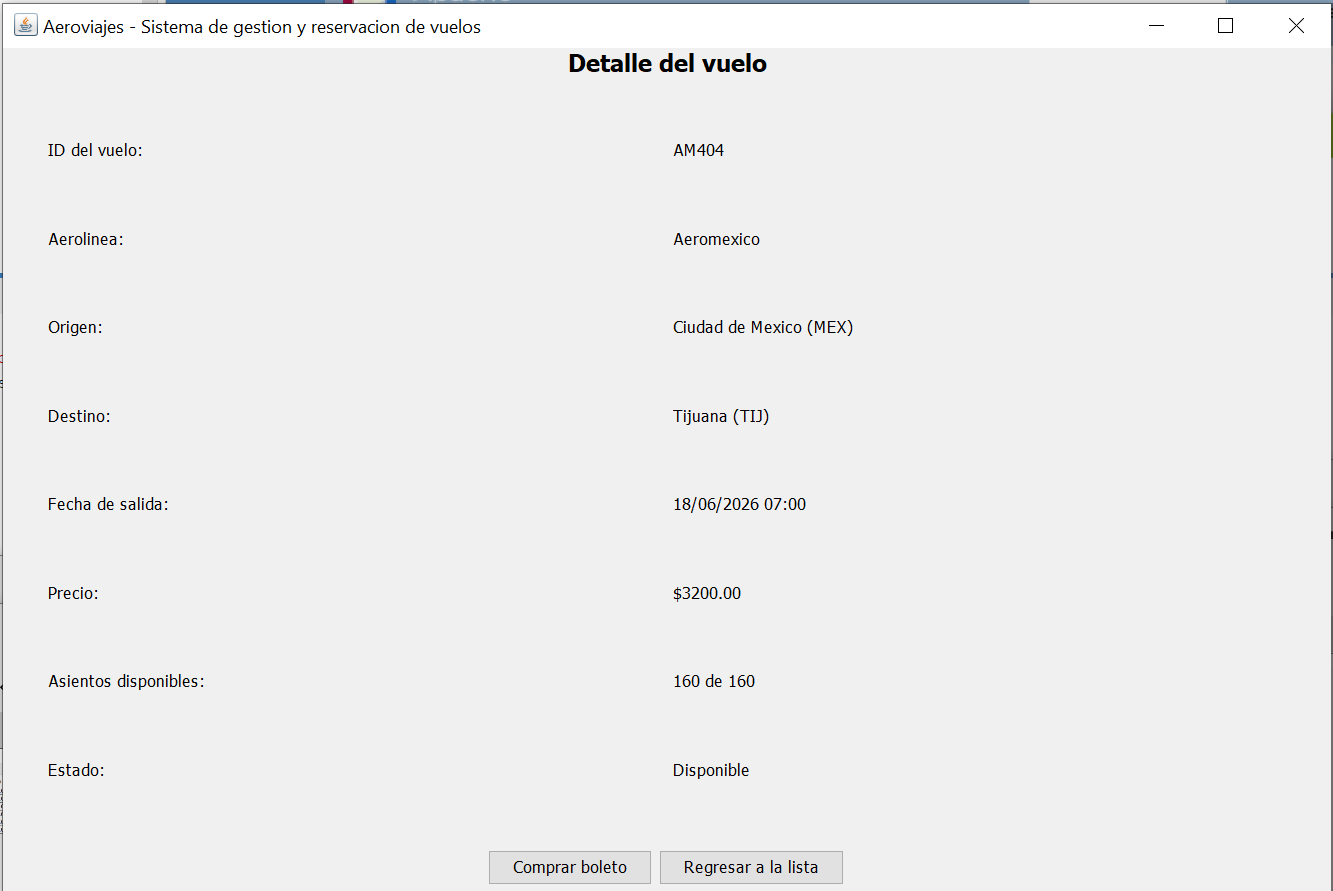
\includegraphics[width=0.8\textwidth]{Aeroviajes 7.png} 
		\caption{Pantalla de detalle del vuelo seleccionado.}
		\label{fig:aeroviajes_7}
	\end{figure}
	
	En esta pantalla el usuario puede revisar toda la información del vuelo antes de confirmar la compra. Si decide proceder, debe pulsar \textbf{``Comprar boleto''}, lo cual desplegará el formulario de \textbf{Datos de Pago}:
	
	\begin{figure}[H]
		\centering
		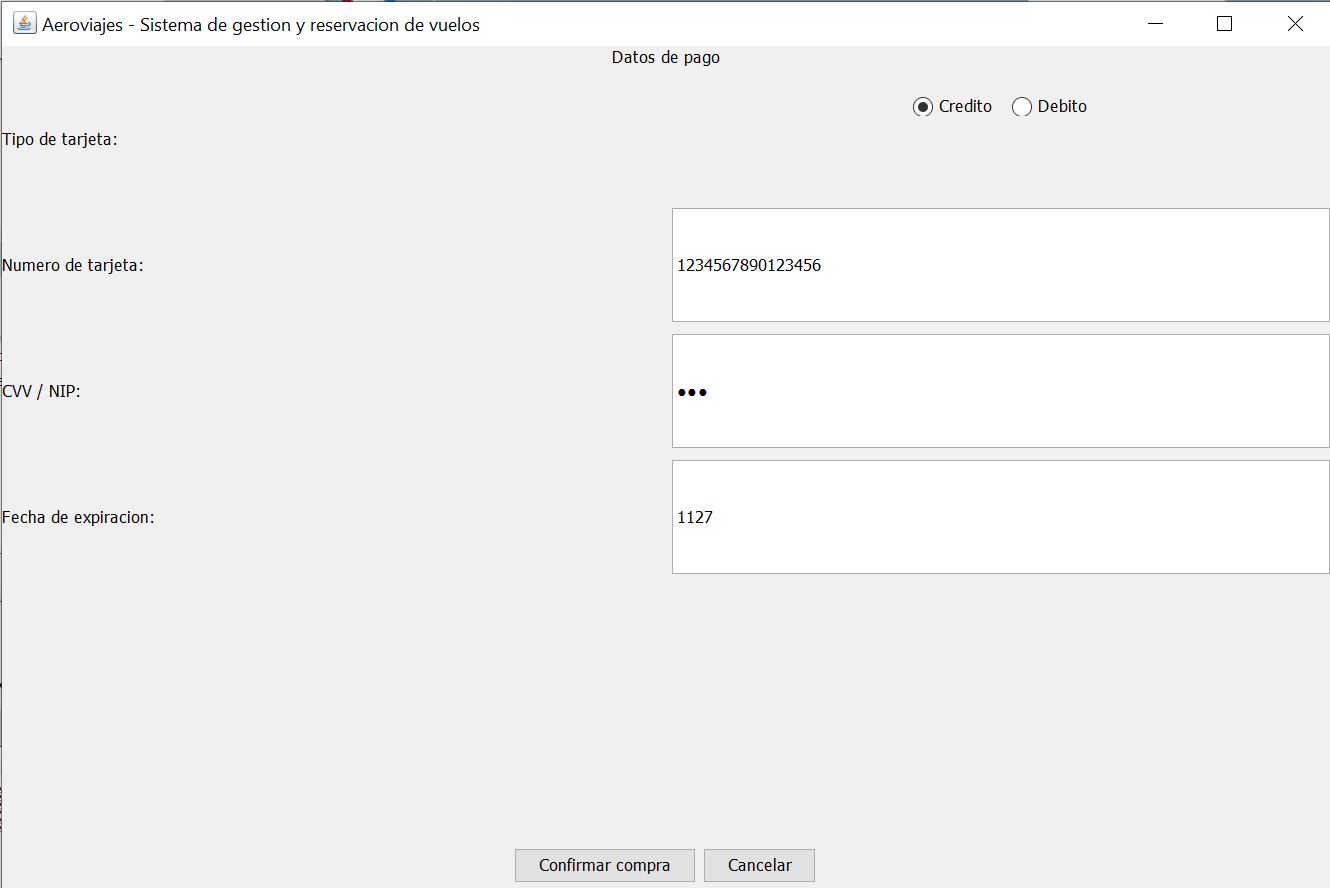
\includegraphics[width=0.7\textwidth]{Aeroviajes 8.png} 
		\caption{Formulario de datos de pago.}
		\label{fig:aeroviajes_8}
	\end{figure}
	
	El usuario debe seleccionar el \textbf{Tipo de tarjeta} (Crédito o Débito) mediante los botones de opción en la parte superior, y completar los tres campos:
	\begin{itemize}
		\item \textbf{Número de tarjeta:} 16 dígitos numéricos sin espacios ni guiones.
		\item \textbf{CVV / NIP:} 3 o 4 dígitos numéricos.
		\item \textbf{Fecha de expiración:} 4 dígitos en formato \texttt{MMAA} (ejemplo: \texttt{1127} para noviembre de 2027).
	\end{itemize}
	
	Tras pulsar \textbf{``Confirmar compra''}, el sistema validará los datos con el algoritmo correspondiente al tipo de tarjeta elegido y, si todo es correcto, generará la reserva. Aparecerá el siguiente diálogo de confirmación:
	
	\begin{figure}[H]
		\centering
		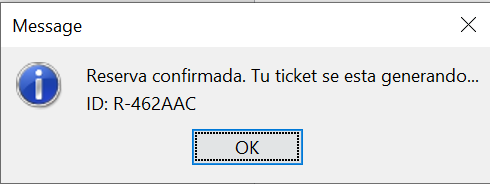
\includegraphics[width=0.6\textwidth]{Aeroviajes 9.png} 
		\caption{Confirmación de reserva exitosa.}
		\label{fig:aeroviajes_9}
	\end{figure}
	
	\begin{quote}
		El mensaje indica que la reserva fue confirmada y el ticket se está generando en segundo plano. Esto significa que el sistema continúa funcionando con normalidad mientras un proceso paralelo crea el archivo del boleto en disco. El usuario no necesita esperar.
	\end{quote}
	
	\subsection{Consulta de Reservas y Descarga del Boleto}
	Para consultar las reservas confirmadas, el usuario debe regresar al menú principal del cliente y pulsar \textbf{``Mis reservas''}:
	
	\begin{figure}[H]
		\centering
		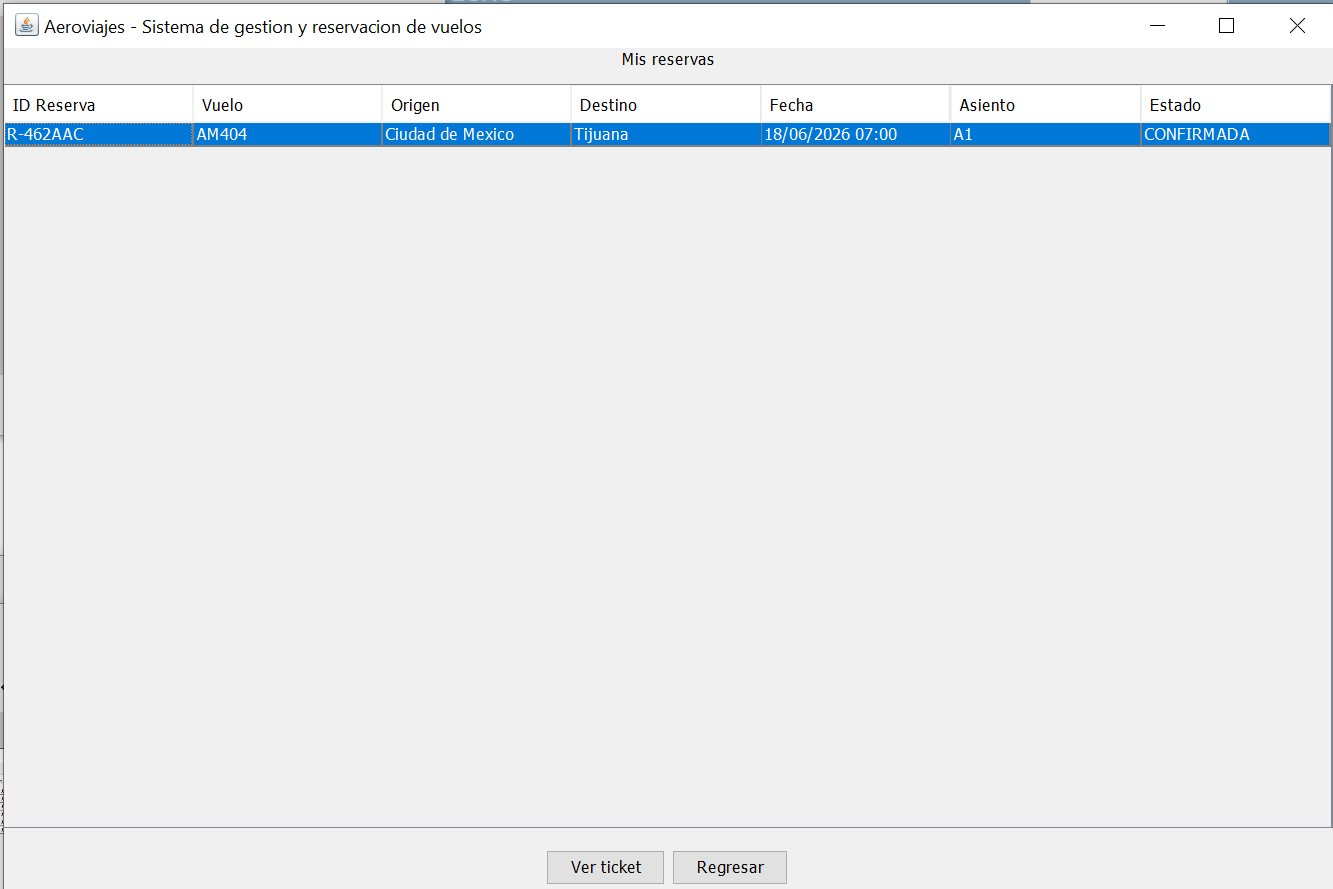
\includegraphics[width=0.85\textwidth]{Aeroviajes 10.png} 
		\caption{Tabla de reservas del cliente.}
		\label{fig:aeroviajes_10}
	\end{figure}
	
	La tabla muestra todas las reservas asociadas al cliente actualmente logueado, con su ID, vuelo, ruta, fecha, asiento y estado. Para ver el boleto completo, el usuario debe seleccionar la fila deseada y pulsar \textbf{``Ver ticket''}:
	
	\begin{figure}[H]
		\centering
		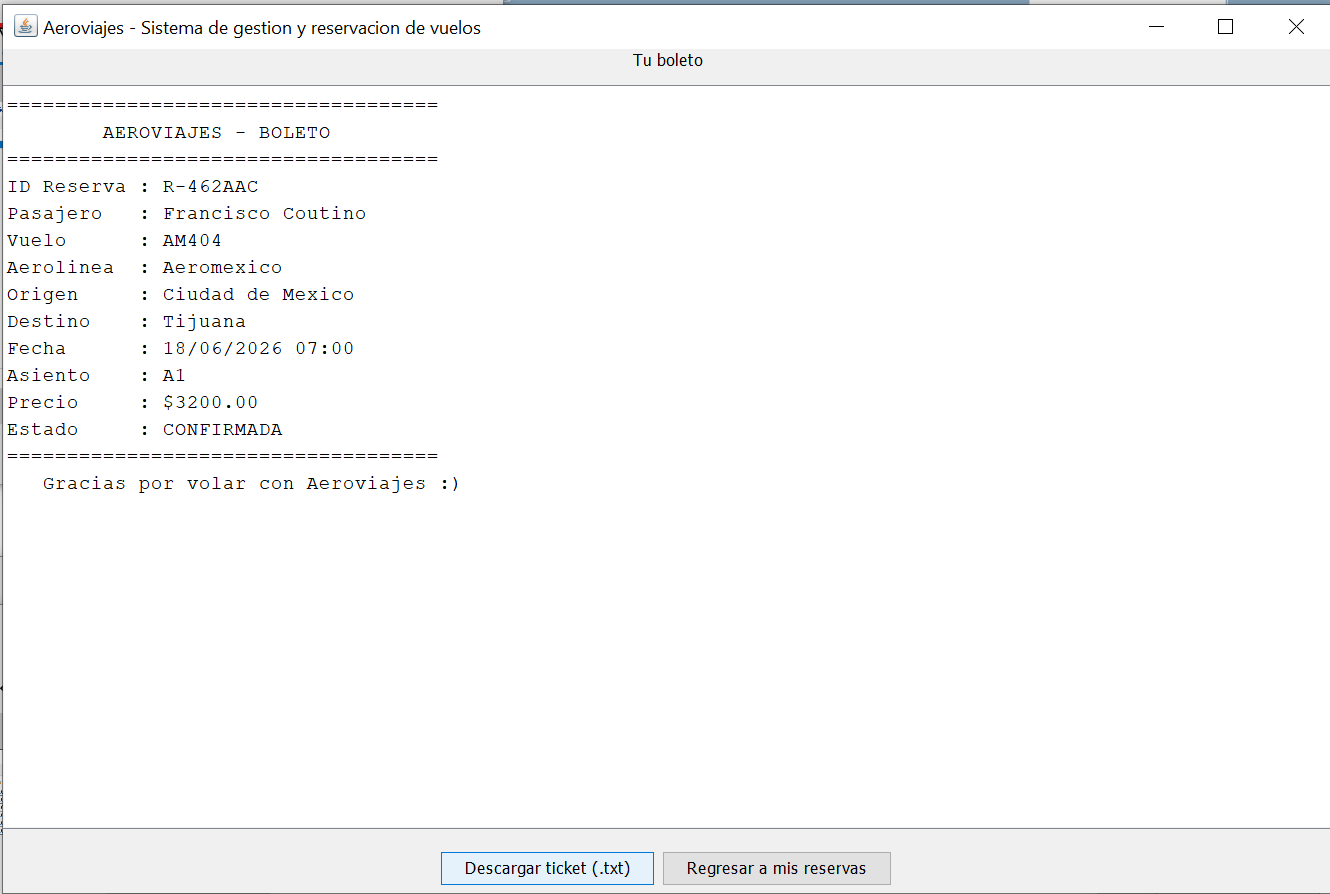
\includegraphics[width=0.8\textwidth]{Aeroviajes 11.png} 
		\caption{Visualización del boleto generado.}
		\label{fig:aeroviajes_11}
	\end{figure}
	
	Esta pantalla muestra el boleto en formato de texto plano, idéntico al archivo \texttt{.txt} que se almacenó en disco. El usuario puede:
	\begin{itemize}
		\item \textbf{Descargar ticket (.txt):} Genera una copia descargable del boleto en la ubicación que el usuario elija.
		\item \textbf{Regresar a mis reservas:} Vuelve a la lista anterior.
	\end{itemize}
	
	% =========================================================================
	% --- SECCIÓN 5: GUÍA DE OPERACIÓN ADMINISTRADOR ---
	% =========================================================================
	\section{Guía de Operación: Administrador}
	Esta sección describe las operaciones disponibles para el usuario administrador, quien tiene control sobre el catálogo de vuelos y los usuarios registrados en el sistema.
	
	\subsection{Acceso al Panel de Administrador}
	Desde la pantalla de bienvenida, el usuario debe pulsar \textbf{``Acceder como administrador''}. Se desplegará la misma pantalla de inicio de sesión que utilizan los clientes, pero esta vez se deben usar las \textbf{credenciales de administrador}:
	
	\begin{figure}[H]
		\centering
		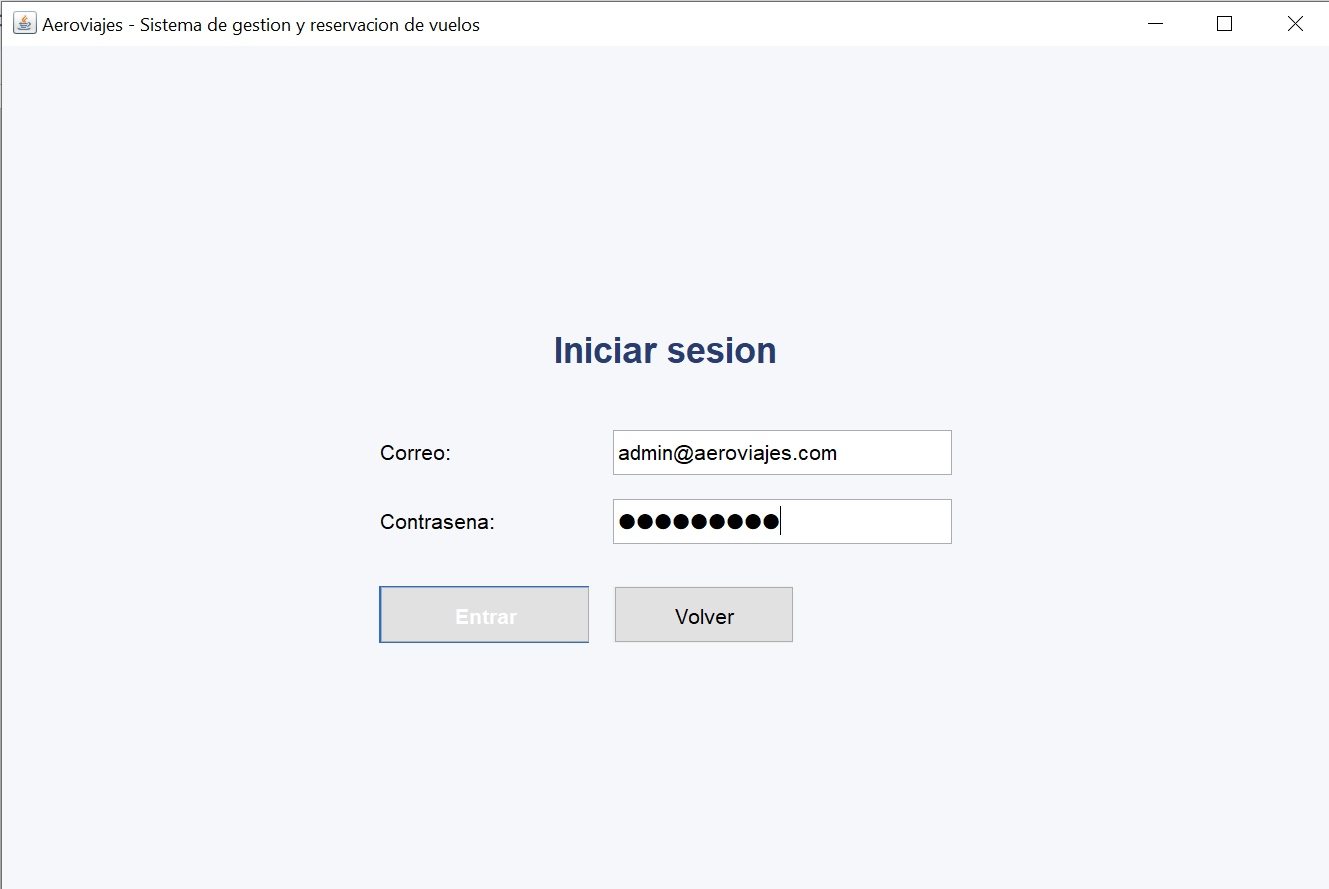
\includegraphics[width=0.7\textwidth]{Aeroviajes 12.png} 
		\caption{Inicio de sesión como administrador.}
		\label{fig:aeroviajes_12}
	\end{figure}
	
	Las credenciales por defecto del administrador (creadas automáticamente la primera vez que se ejecuta el sistema) son:
	\begin{itemize}
		\item \textbf{Correo:} \texttt{admin@aeroviajes.com}
		\item \textbf{Contraseña:} \texttt{Admin123!}
	\end{itemize}
	
	Tras autenticar correctamente, el sistema redirige al \textbf{Panel de Administrador}:
	
	\begin{figure}[H]
		\centering
		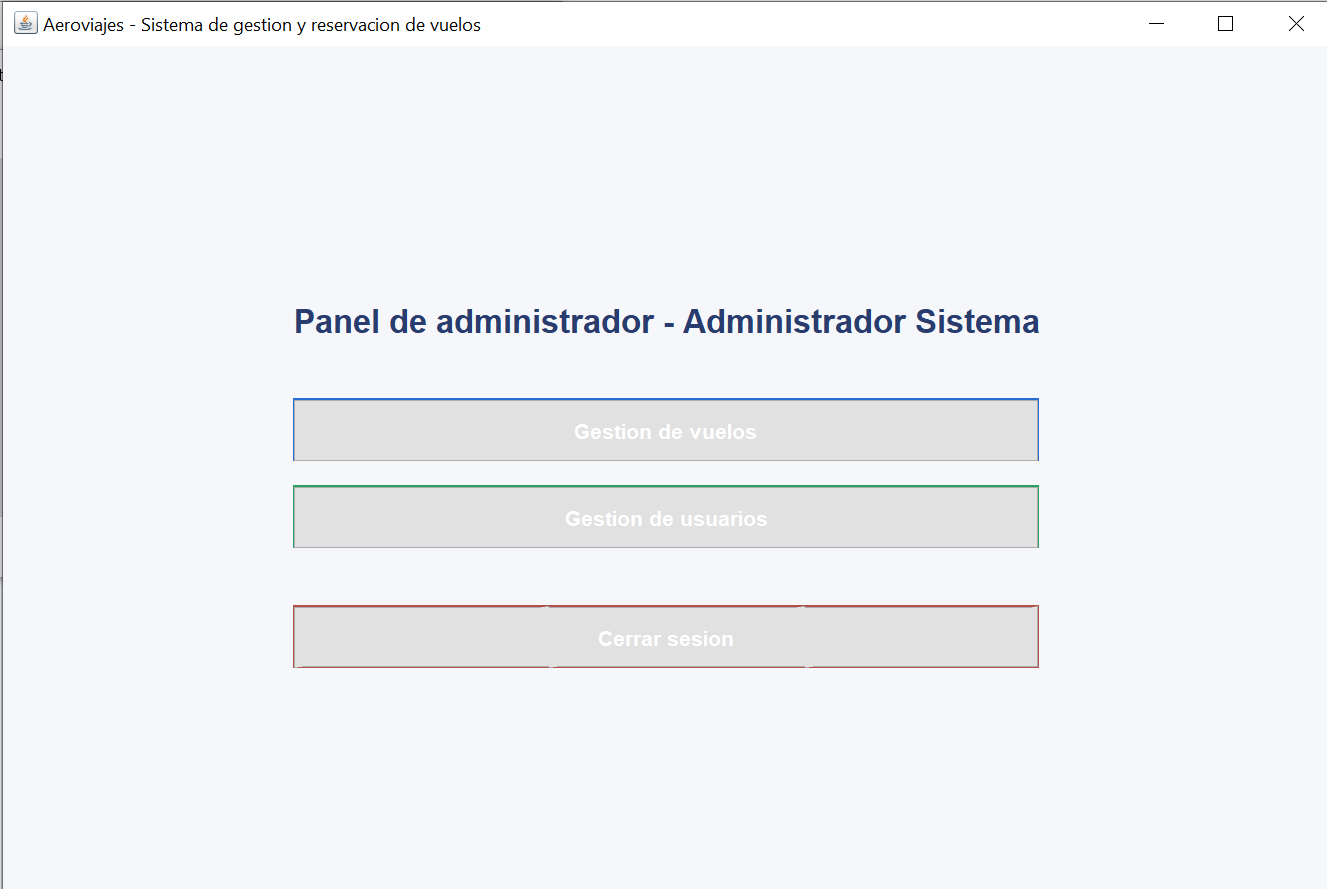
\includegraphics[width=0.8\textwidth]{Aeroviajes 13.png} 
		\caption{Panel principal del administrador.}
		\label{fig:aeroviajes_13}
	\end{figure}
	
	Las tres opciones disponibles son:
	\begin{itemize}
		\item \textbf{Gestión de vuelos:} Permite agregar, eliminar y consultar todos los vuelos del catálogo.
		\item \textbf{Gestión de usuarios:} Permite consultar y eliminar a los usuarios registrados.
		\item \textbf{Cerrar sesión:} Termina la sesión activa.
	\end{itemize}
	
	\subsection{Gestión de Vuelos}
	Al pulsar \textbf{``Gestión de vuelos''}, el sistema despliega la tabla completa de vuelos del catálogo (incluyendo los que ya no tienen asientos disponibles), junto con el formulario para agregar uno nuevo:
	
	\begin{figure}[H]
		\centering
		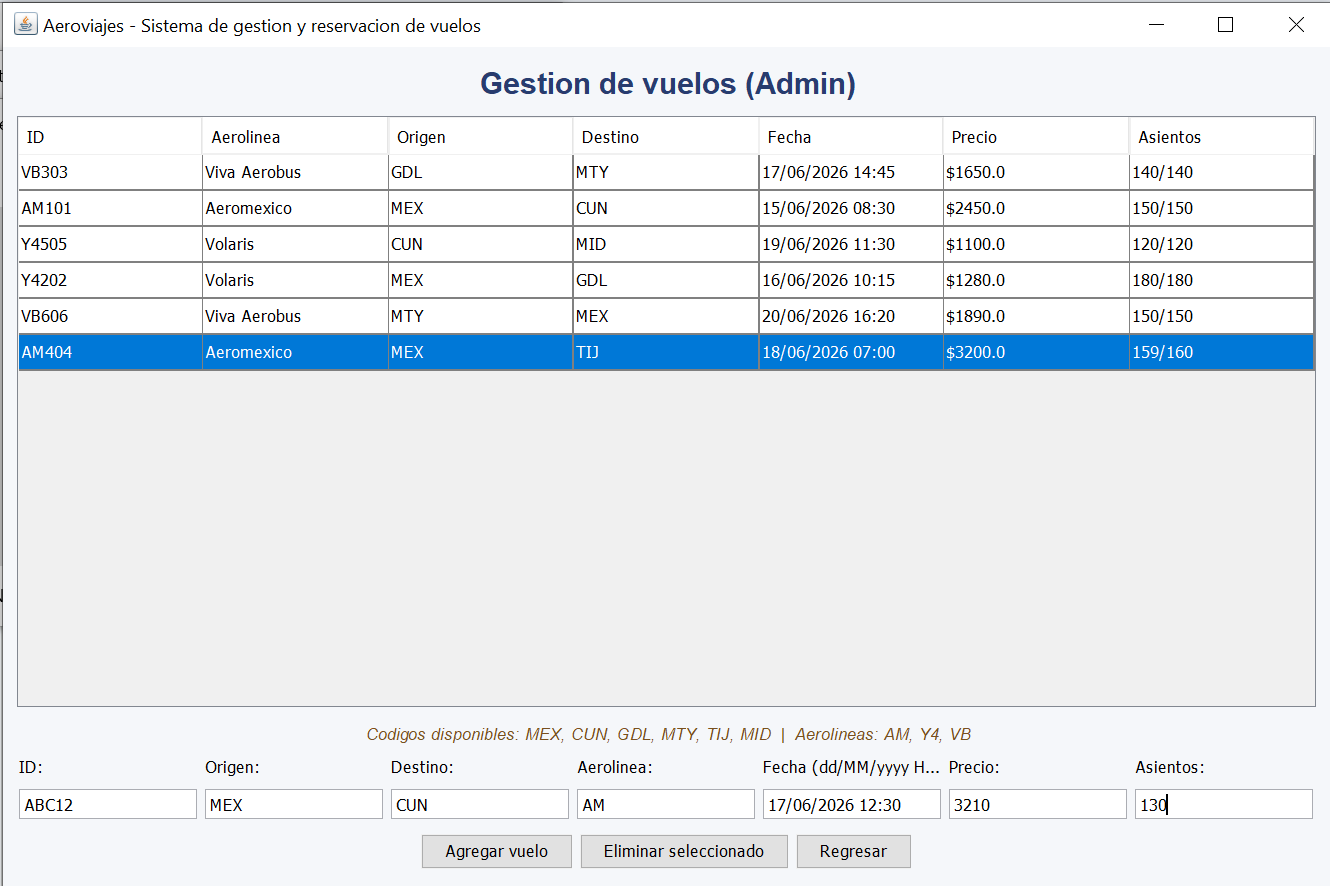
\includegraphics[width=0.85\textwidth]{Aeroviajes 14.png} 
		\caption{Pantalla de gestión de vuelos.}
		\label{fig:aeroviajes_14}
	\end{figure}
	
	\textbf{Para agregar un vuelo nuevo,} el administrador debe completar los campos en la parte inferior:
	\begin{itemize}
		\item \textbf{ID:} Identificador único del vuelo (ej. \texttt{ABC12}). Si se deja vacío, el sistema lo genera automáticamente.
		\item \textbf{Origen y Destino:} Código IATA de tres letras del aeropuerto. Solo se aceptan los códigos pre-cargados en el sistema: \texttt{MEX, CUN, GDL, MTY, TIJ, MID}.
		\item \textbf{Aerolínea:} Código de la aerolínea. Solo se aceptan los códigos pre-cargados: \texttt{AM} (Aeromexico), \texttt{Y4} (Volaris), \texttt{VB} (Viva Aerobus).
		\item \textbf{Fecha:} Fecha y hora de salida en formato exacto \texttt{dd/MM/yyyy HH:mm} (ejemplo: \texttt{17/06/2026 12:30}).
		\item \textbf{Precio:} Costo del boleto en pesos. Solo número decimal.
		\item \textbf{Asientos:} Capacidad total del vuelo. Solo número entero positivo.
	\end{itemize}
	
	Tras pulsar \textbf{``Agregar vuelo''}, el sistema valida los datos, persiste el vuelo en disco y muestra una confirmación:
	
	\begin{figure}[H]
		\centering
		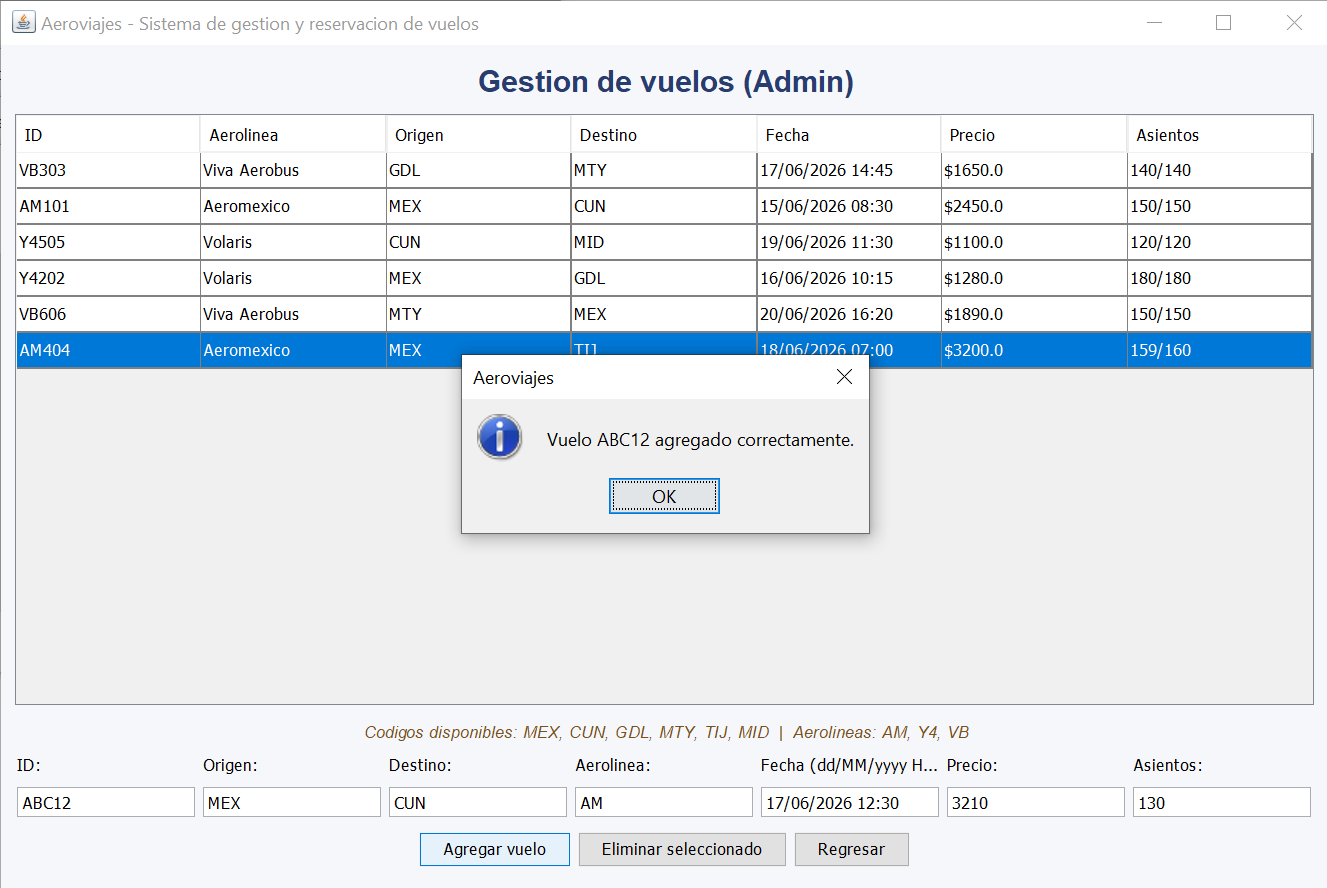
\includegraphics[width=0.6\textwidth]{Aeroviajes 15.png} 
		\caption{Confirmación de vuelo agregado correctamente.}
		\label{fig:aeroviajes_15}
	\end{figure}
	
	\textbf{Para eliminar un vuelo,} el administrador debe seleccionar la fila correspondiente en la tabla y pulsar \textbf{``Eliminar seleccionado''}. El sistema solicitará confirmación antes de proceder. Una vez eliminado, el vuelo desaparece tanto de la tabla como de los archivos persistidos.
	
	\subsection{Gestión de Usuarios}
	Al pulsar \textbf{``Gestión de usuarios''} desde el panel principal del administrador, se despliega la tabla con todos los usuarios registrados en el sistema:
	
	\begin{figure}[H]
		\centering
		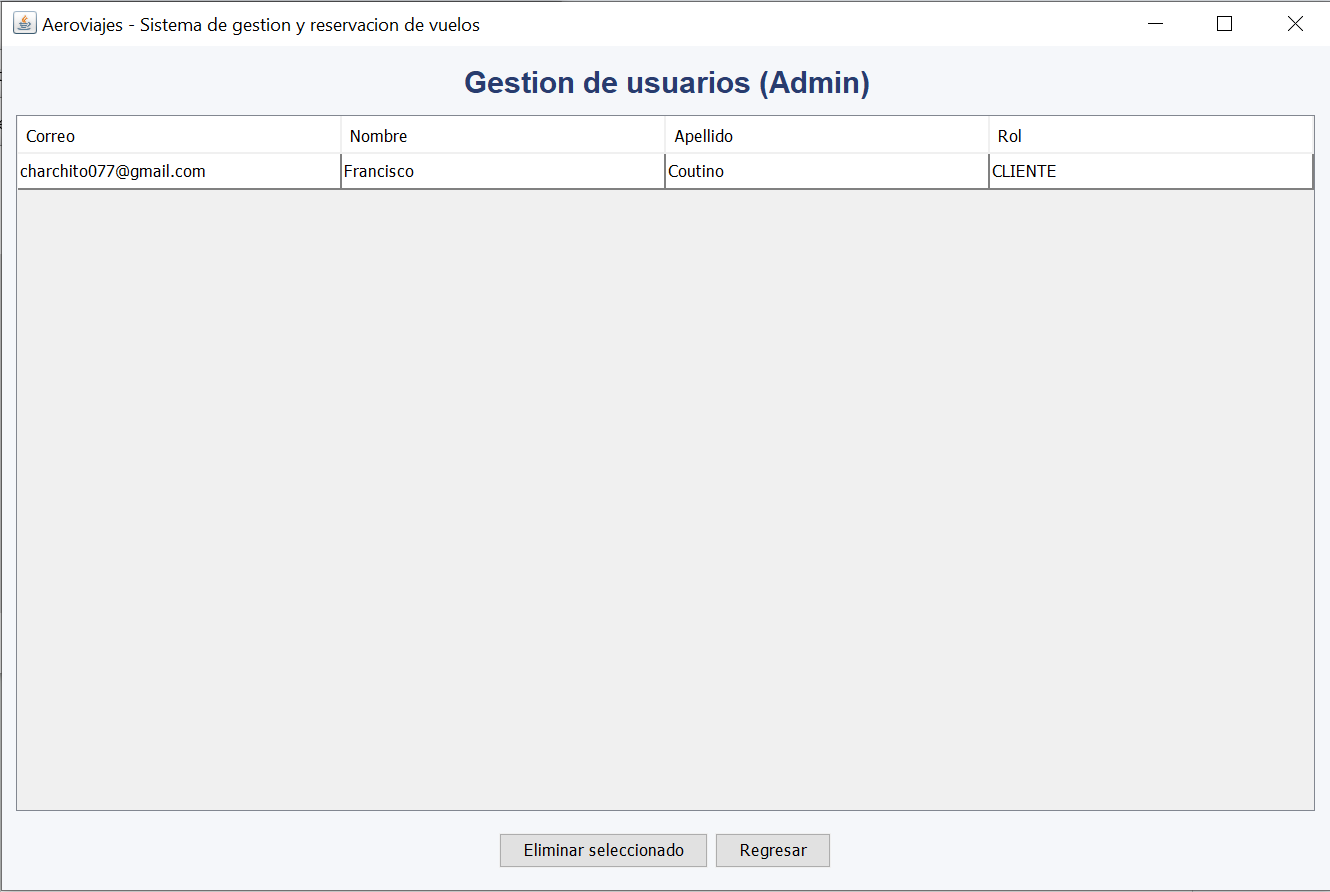
\includegraphics[width=0.85\textwidth]{Aeroviajes 16.png} 
		\caption{Pantalla de gestión de usuarios.}
		\label{fig:aeroviajes_16}
	\end{figure}
	
	La tabla muestra el correo, nombre, apellido y rol (\texttt{CLIENTE} o \texttt{ADMINISTRADOR}) de cada usuario. Para eliminar a un usuario, el administrador debe seleccionar la fila correspondiente y pulsar \textbf{``Eliminar seleccionado''}.
	
	\begin{quote}
		\textbf{Nota de seguridad:} El sistema impide que el administrador elimine su propia cuenta mientras está logueado, para evitar quedar bloqueado fuera del panel administrativo.
	\end{quote}
	
	% =========================================================================
	% --- SECCIÓN 6: CIERRE SEGURO DEL PROGRAMA ---
	% =========================================================================
	\section{Cierre Seguro del Programa}
	Para cerrar el programa de manera segura sin pérdida de datos, el usuario debe:
	\begin{enumerate}
		\item Cerrar primero la sesión activa pulsando \textbf{``Cerrar sesión''} desde el menú correspondiente (cliente o administrador).
		\item Cerrar la ventana principal del programa con el botón \textbf{X} en la esquina superior derecha.
	\end{enumerate}
	El sistema persiste automáticamente todos los cambios en disco (usuarios, vuelos, reservas) después de cada operación, por lo que en condiciones normales no debe haber pérdida de información ni siquiera con un cierre abrupto. Sin embargo, se recomienda siempre cerrar la sesión correctamente.
	
% =========================================================================
% --- SECCIÓN 7: ADVERTENCIAS CRÍTICAS ---
% =========================================================================
\section{Advertencias Críticas y Prevención de Fallos}
El sistema cuenta con validaciones lógicas robustas, manejo de excepciones en cada operación e interfaz gráfica que captura los errores antes de que afecten la ejecución. Sin embargo, existen ciertas condiciones externas al programa y comportamientos del usuario que el operador debe conocer para evitar resultados inesperados.

\begin{tcolorbox}[colback=lightgray, colframe=warningred, title=\textbf{1. ERROR FATAL: Manipulación Manual de los Archivos de Datos}]
	La causa más común de un \textbf{cierre abrupto del programa} es la manipulación externa de los archivos generados por el sistema, ubicados en la carpeta \texttt{data/} del proyecto:
	\begin{itemize}
		\item \texttt{data/usuarios.dat}
		\item \texttt{data/vuelos.dat}
		\item \texttt{data/reservas.dat}
		\item \texttt{data/tickets/*.txt}
	\end{itemize}
	Estos archivos almacenan datos serializados en formato binario. Las siguientes acciones provocarán el cierre inmediato del programa (o impedirán que arranque):
	\begin{itemize}
		\item \textbf{Editar los archivos \texttt{.dat} con cualquier editor de texto} (Bloc de notas, VS Code, Notepad++). La serialización binaria de Java se corrompe al modificarse, y al intentar cargarla el sistema lanza \texttt{StreamCorruptedException} o \texttt{InvalidClassException}, terminando la ejecución.
		\item \textbf{Eliminar archivos \texttt{.dat} mientras el programa está corriendo.} Si el sistema intenta persistir datos y el directorio fue modificado externamente, se lanza \texttt{IOException} no recuperable.
		\item \textbf{Cerrar el programa con \texttt{Ctrl+C} desde la consola de NetBeans} en medio de una operación de guardado. Los archivos pueden quedar truncados y al siguiente arranque no podrán cargarse.
	\end{itemize}
	\textbf{Solución si esto ocurre:} Borrar por completo la carpeta \texttt{data/} y reiniciar el programa. El sistema regenerará automáticamente los archivos, creará el administrador por defecto y sembrará 6 vuelos de muestra.
\end{tcolorbox}

\begin{tcolorbox}[colback=lightgray, colframe=warningred, title=\textbf{2. ERROR FATAL: Falta de Permisos o Espacio en Disco}]
	El programa requiere permisos de \textbf{escritura} en la carpeta del proyecto. Si estos permisos son denegados (por antivirus, por estar el proyecto en una ruta protegida como \texttt{Archivos de programa}, o por una unidad de red sin permisos), el sistema lanzará \texttt{IOException} al intentar persistir cualquier operación.
	
	De igual forma, si el disco duro se queda \textbf{sin espacio libre} durante una operación de guardado, el programa puede cerrarse abruptamente.
	
	\textbf{Recomendación:} Mantener el proyecto en una carpeta del usuario (por ejemplo \texttt{C:\textbackslash Users\textbackslash TuUsuario\textbackslash} o el Escritorio) y verificar que el antivirus no tenga al ejecutable de Java en cuarentena.
\end{tcolorbox}

\begin{tcolorbox}[colback=lightgray, colframe=primary, title=\textbf{3. ADVERTENCIA LÓGICA: Operaciones Rechazadas por el Sistema}]
	A diferencia de los errores fatales, las siguientes situaciones \textbf{no cierran el programa} — el sistema cancela la operación y muestra un mensaje de error amigable, permitiendo al usuario corregir y continuar:
	\begin{itemize}
		\item \textbf{Formato de fecha incorrecto al agregar un vuelo.} El sistema espera exactamente \texttt{dd/MM/yyyy HH:mm} (ejemplo: \texttt{17/06/2026 12:30}). Formatos como \texttt{2026-06-17}, \texttt{17/Junio/2026} u horarios \texttt{8:30 AM} serán rechazados.
		\item \textbf{Caracteres no numéricos en campos de precio, asientos, número de tarjeta o CVV.} Estos campos solo aceptan dígitos. Símbolos como \texttt{\$} o comas como separadores de miles (escribir \texttt{1,500.50} en lugar de \texttt{1500.50}) causarán el rechazo de la operación.
		\item \textbf{Correo ya registrado.} No se puede registrar a un cliente con un correo que ya existe en el sistema. El correo es la clave única.
		\item \textbf{Credenciales incorrectas en el inicio de sesión.} El sistema mostrará un mensaje específico (``No existe un usuario con ese correo'' o ``Contraseña incorrecta'') sin cerrar la aplicación.
		\item \textbf{Acceso indebido a paneles de administrador.} Si un cliente intentara —por cualquier medio— acceder a operaciones de administrador, el patrón Proxy implementado lanza una excepción de autenticación que se traduce en un mensaje de error.
	\end{itemize}
\end{tcolorbox}

\subsection{Restricciones de Valores No Válidos}
El sistema bloquea y cancela la operación mostrando un mensaje informativo si el usuario intenta:
\begin{itemize}
	\item Registrarse con un correo sin formato válido (debe contener \texttt{@} y un dominio con punto, ej. \texttt{usuario@dominio.com}).
	\item Registrarse con un nombre o apellido que contenga números o símbolos. Solo se aceptan letras y espacios, entre 2 y 50 caracteres.
	\item Agregar un vuelo con un \textbf{código IATA de origen o destino no registrado}. Solo se aceptan los códigos pre-cargados: \texttt{MEX, CUN, GDL, MTY, TIJ, MID}.
	\item Agregar un vuelo con un \textbf{código de aerolínea no registrado}. Solo se aceptan: \texttt{AM, Y4, VB}.
	\item Introducir un precio menor o igual a cero.
	\item Introducir una cantidad de asientos menor o igual a cero.
	\item Comprar un boleto en un vuelo sin asientos disponibles.
	\item Eliminar al usuario administrador actualmente logueado (medida de seguridad para evitar quedar bloqueado del panel).
\end{itemize}

Para una experiencia óptima, se recomienda al usuario respetar los formatos indicados en cada formulario y prestar atención a los mensajes que el sistema despliega tras cada operación. \textbf{Mientras no se manipulen externamente los archivos de la carpeta \texttt{data/}, el programa se mantiene estable durante toda la sesión.}
\end{document}